\clearpage
\section{Analysis}
\label{sec:empirical_findings}

With the information of code commits, \textit{GitHub} projects' metrics, issue communication and user events (over time) we can verify the following hypotheses:

\begin{itemize}
    \item [\textbf{H 1}] Firm employees' participation affects the participation of external developers
		\begin{itemize}
			\item [\textbf{H 1.1}] If firm employees contribute source code more often, external developers do as well
			\item [\textbf{H 1.2}] If firm employees participate more often on issue threads, external developers do as well
		\end{itemize}
    \item [\textbf{H 2}] Firm employees' participation (in the beginning) affects the (later) success of firm-initiated open source projects
		\begin{itemize}
			\item [\textbf{H 2.1}] If firm employees contribute source code more often in the beginning, the project gets more successful
		\end{itemize}
		\item [\textbf{H 3}] If firm employees' contribution share is higher overall the more likely the project is popular
\end{itemize}


\subsection{Terms and Definitions}
\label{sec:lm_terms_and_definitions}
\begin{itemize}
	\item [\textbf{Younger Projects:}] Projects that are younger than 1 year (\textless 365 days)
	\item [\textbf{Older Projects:}] Projects that are older than 1 year (\textgreater= 365 days)
	\item [\textbf{Top Projects:}] Projects that were found in the first 1000 most popular projects of a programming language (can be 1 or 0, see below for mathematical definition)
	\item [\textbf{Residual Projects}] Projects that were \textit{not} found in the 1000 most popular projects for a programming language \footnote{"Top Projects" and "Residual Projects" together build the set of relevant projects}
	\item [\textbf{Ratio}] Code commit share of firm employed developers to external developers (normalized value between 0 and 1)
\end{itemize}

\begin{align}
\mathit{Ratio} =
	\begin{cases}
		1         & \quad \text{if repository is maintained to 100\% by firm employed developers only}\\
		0         & \quad \text{if repository is maintained to 0\% by firm developers (i.e. 100\% external developers)}\\
		\in (0,1) & \quad \text{else}\\
	\end{cases}
\end{align}

\begin{align}
\mathit{Top \ Project} =
	\begin{cases}
		1         & \quad \text{if is found in search of 1000 most starred projects of the 10 selected Languages}\\
		0         & \quad \text{else}\\
	\end{cases}
\end{align}

\subsection{Slopes and Dots (on plot figures)}
\label{sec:lm_plots_description}
\begin{itemize}
	\item [\textbf{Yellow-Solid}]
	$\vcenter{\hbox{\includegraphics[scale=0.05]{../hypotheses/legend/yellow_slope.png}}}$
	Correlation coefficient for the influence of code commits from firm employed developers on external developers (via OLS)

	\item [\textbf{Blue-Dashed}]
	$\vcenter{\hbox{\includegraphics[scale=0.045]{../hypotheses/legend/blue_slope.png}}}$
	Correlation coefficient for the influence of code commits from external developers on firm employed developers (via OLS) \footnote{actually x- and y-axis must be reverted to illustrate external impact on firm employed developers, but for the sake of simplicity blue and yellow slopes share one plot here}

	\item [\textbf{Grey Dots}] $\vcenter{\hbox{\includegraphics[scale=0.07]{../hypotheses/legend/dots.png}}}$
	Number of code contribution by firm employed developers (x-axis) and external developers (y-axis)

\end{itemize}

\subsection{H 1: Firm employees' participation affects the participation of external developers}
\subsection{H 1.1: If firm employees contribute source code more often, external developers do as well}

\subsubsection{H 1.1: Models and Terminology}

The following linear models (using OLS) examine the influence of code contribution by firm employed developers on external developers and vice versa.

Every project is represented by a dot and plotted through number of code contributions by firm employed developers (x-axis) against number of code contributions by external developers (y-axis). The influence of firm employed developers' participation (independent) on external developers' participation (dependent) is represented by the solid yellow slope and defined in the models 1.1, 1.3, 1.5, 1.7, 1.9, 1.11 and 1.13. Conversely, the influence of external developers' participation (independent) on firm employed developers' participation (dependent) is represented by the dashed blue slope and defined in the models 1.2, 1.4, 1.6, 1.8, 1.10, 1.12 and 1.14. For better understanding see plots \ref{fig:hyp1_model_1-2} - \ref{fig:hyp1_model_11-12} \footnote{plot for model 1.12 and 1.13 (internal and external commits on younger Residual Projects) was omitted since there is no significant correlation, as noted in table \ref{tbl:regression_table_1.1.13-1.1.14}} and regression results i.a. in table \ref{tbl:hyp1_model_1-4} (page \pageref{tbl:hyp1_model_1-4} and page \pageref{sec:regression_tables_h1.1}ff).

\begin{itemize}
	\item [\textbf{int. commits / internal commits:}] Number of code contributions by firm employed developers
	\item [\textbf{ext. commits / external commits:}] Number of code contributions by external developers
\end{itemize}

See section \ref{sec:lm_terms_and_definitions} and \ref{sec:lm_plots_description} for further explanation of terms, definitions and plots.

\textit{R} code will be used to describe the models \footnote{all analyses are made in \textit{R}; so the models are taken from the source code} since it's a bit handier to describe than in mathematical notation. \textit{See listing \ref{lst:lm_h1.1} on page \pageref{lst:lm_h1.1} for details.}

\subsubsection{H 1.1: Plots}

See page \pageref{sec:h_1.1_plots} for plots.

% \clearpage
\subsubsection{H 1.1: Regression Tables}

Additional regression tables can be found in chapter \ref{sec:regression_tables_h1.1}, page \pageref{tbl:regression_table_1.1.5-1.1.7} - \pageref{tbl:regression_table_1.1.13-1.1.14} (table \ref{tbl:regression_table_1.1.5-1.1.7}, \ref{tbl:regression_table_1.1.9-1.1.12} and \ref{tbl:regression_table_1.1.13-1.1.14}).

\begin{table}[!h] \centering
  \scriptsize{
	  
% Table created by stargazer v.5.2 by Marek Hlavac, Harvard University. E-mail: hlavac at fas.harvard.edu
% Date and time: Tue, Mar 15, 2016 - 11:34:21
\begin{tabular}{@{\extracolsep{5pt}}lcccc}
\\[-1.8ex]\hline
\hline \\[-1.8ex]
 & \multicolumn{4}{c}{\textit{Dependent variable:}} \\
\cline{2-5}
\\[-1.8ex] & ext. commits & int. commits & ext. commits & int. commits \\
\\[-1.8ex] & (1.1.1) & (1.1.2) & (1.1.3) & (1.1.4)\\
\hline \\[-1.8ex]
 int. commits & 0.999$^{***}$ &  & 0.794$^{***}$ &  \\
  & (0.091) &  & (0.040) &  \\
  & & & & \\
 ext. commits &  & 0.034$^{***}$ &  & 0.492$^{***}$ \\
  &  & (0.003) &  & (0.025) \\
  & & & & \\
 Constant & 247.010$^{*}$ & 233.808$^{***}$ & 48.746 & 540.463$^{***}$ \\
  & (138.107) & (25.282) & (141.371) & (109.104) \\
  & & & & \\
\hline \\[-1.8ex]
Observations & 3,419 & 3,419 & 610 & 610 \\
R$^{2}$ & 0.034 & 0.034 & 0.390 & 0.390 \\
Adjusted R$^{2}$ & 0.034 & 0.034 & 0.389 & 0.389 \\
Residual Std. Error & 7,964.959 (df = 3417) & 1,475.494 (df = 3417) & 3,368.299 (df = 608) & 2,651.187 (df = 608) \\
F Statistic & 121.248$^{***}$ (df = 1; 3417) & 121.248$^{***}$ (df = 1; 3417) & 388.882$^{***}$ (df = 1; 608) & 388.882$^{***}$ (df = 1; 608) \\
\hline
\hline \\[-1.8ex]
\textit{Note:}  & \multicolumn{4}{r}{$^{*}$p$<$0.1; $^{**}$p$<$0.05; $^{***}$p$<$0.01} \\
\end{tabular}

  }
	\caption{Influence of internal commits on external commits (and v.v.) on "All Projects" (Model 1.1.1 - 1.1.2) and "Top Projects" (Model 1.1.3 - 1.1.4)}
	\label{tbl:hyp1_model_1-4}
\end{table}

\clearpage
\subsubsection{H 1.1: Results and Interpretation}

\textbf{The regression results confirm the hypothesis:} \footnote{Except model 1.1.13 and 1.1.14 (influence of code contribution on young residual projects, i.e. new and unknown projects of firms). But we have to be consider, that model 1.1.13 and 1.1.14 are using the smallest subset of 909 observations, which may cause the poor fitting among other things.} If firm employed developers contribute more source code, external developers contribute more source code as well.

The reversed impact (i.e. influence of code contributions from external developers on contributions of firm employed developers) is also existing - except for (older) top projects - but essentially weaker in all cases. The distance between the impact of internal developers on external developers and the other way round decreases if projects are more popular (i.e. "Top Projects") \footnote{on "Top Projects" externals' participation has a high positive impact on internal developers as well}. This indicates, that the biggest positive impact of internal developers' participation on external developers' participation is reached in not well-known (and younger) projects.

\textbf{The number of code commits by firm employed developers have a high positive significant influence on the number of code commits by external developers. The impact of code commits by external developers on firm employed developers is also positive, but significant lower - especially in not well-known projects.}

\newpage

\subsection{H 1.2: If firm employees participate more often on issue threads, external developers do as well}

\subsubsection{H 1.2.1: Models and Terminology for Issues}

We observe the number of created (i.e. opened) issues by \textit{GitHub} users. With linear regression we want to determine the influence of the participation of firm employed developers on the participation of external \textit{GitHub} users and vice versa. Neither we consider the content size (i.e. how much the user actually wrote) nor do we rate the quality of an issue.

\begin{itemize}
	\item [\textbf{issues by int. users:}] Number of issues created by firm employed developers / \textit{GitHub} users
	\item [\textbf{issues by ext. users:}] Number of issues created by external developers / \textit{GitHub} users
\end{itemize}

See section \ref{sec:lm_terms_and_definitions} and \ref{sec:lm_plots_description} (page \pageref{sec:lm_terms_and_definitions} and \pageref{sec:lm_plots_description}) for further explanation of terms, definitions and plots.

% Graphic Export: 5x8 inch
\textit{See listing \ref{lst:lm_h1.2} on page \pageref{lst:lm_h1.2} for defined models in R code.}

\subsubsection{H 1.2.1: Plots for Issues}

See page \pageref{sec:h_1.2.1_plots} for plots.

% \clearpage
\subsubsection{H 1.2.1: Regression Tables for Issues}

Additional regression tables can be found in \ref{tbl:regression_table_1.2.5-1.2.8}, page \pageref{tbl:regression_table_1.2.5-1.2.8} -  \pageref{tbl:regression_table_1.2.13-1.2.14} (table \ref{tbl:regression_table_1.2.5-1.2.8}, \ref{tbl:regression_table_1.2.9-1.2.10} and \ref{tbl:regression_table_1.2.13-1.2.14}).

\begin{table}[!h] \centering
  \scriptsize{
	  
% Table created by stargazer v.5.2 by Marek Hlavac, Harvard University. E-mail: hlavac at fas.harvard.edu
% Date and time: Tue, Mar 15, 2016 - 20:38:55
\begin{tabular}{@{\extracolsep{5pt}}lcccc}
\\[-1.8ex]\hline
\hline \\[-1.8ex]
 & \multicolumn{4}{c}{\textit{Dependent variable:}} \\
\cline{2-5}
\\[-1.8ex] & issues by ext. users & issues by firm empl. users & issues by ext. users & issues by firm empl. users \\
\\[-1.8ex] & (1.2.1) & (1.2.2) & (1.2.3) & (1.2.4)\\
\hline \\[-1.8ex]
 issues by firm empl. users & 23.800$^{***}$ &  & 33.598$^{***}$ &  \\
  & (0.867) &  & (2.443) &  \\
  & & & & \\
 issues by ext. users &  & 0.009$^{***}$ &  & 0.008$^{***}$ \\
  &  & (0.0003) &  & (0.001) \\
  & & & & \\
 Constant & 70.842$^{***}$ & 0.704$^{***}$ & 228.113$^{***}$ & 2.252$^{***}$ \\
  & (7.446) & (0.143) & (38.219) & (0.599) \\
  & & & & \\
\hline \\[-1.8ex]
Observations & 2,935 & 2,935 & 523 & 523 \\
R$^{2}$ & 0.205 & 0.205 & 0.266 & 0.266 \\
Adjusted R$^{2}$ & 0.204 & 0.204 & 0.265 & 0.265 \\
Residual Std. Error & 395.887 (df = 2933) & 7.523 (df = 2933) & 817.527 (df = 521) & 12.557 (df = 521) \\
F Statistic & 754.343$^{***}$ (df = 1; 2933) & 754.343$^{***}$ (df = 1; 2933) & 189.129$^{***}$ (df = 1; 521) & 189.129$^{***}$ (df = 1; 521) \\
\hline
\hline \\[-1.8ex]
\textit{Note:}  & \multicolumn{4}{r}{$^{*}$p$<$0.1; $^{**}$p$<$0.05; $^{***}$p$<$0.01} \\
\end{tabular}

  }
	\caption{Impact of issue participation by firm employed developers on external users (and v.v.) in "All Projects" (Model 1.2.1 - 1.2.2) and "Top Projects" (Model 1.2.3 - 1.2.4)}
  \label{tbl:regression_table_1.2.1-1.2.4}
\end{table}

\clearpage
\subsubsection{H 1.2.2: Models for Issues' Comments}
\label{sec:h1.2.2_models}

Every issue contains comments which enables discussion between users. Beside the number of comments per issue we consider the size of involvement for every user by measuring the size of written text. Every character of a comment is taken into account and finally add up to obtain a share of content contribution. This implies that if (for example) a firm employed developer writes 400 characters long comments in total inside an issue thread with all comments together having a size of 1,200 characters, the content share of the firm employed developer would be $\frac{1}{3}$. We also use the number of issue comments as unit of measurement.

Every dot represents an issue with it's comments and is plotted through \textit{number of issue comments by firm employee / developer} (x-axis) against \textit{number of issue comments by external users} (y-axis). See section \ref{sec:lm_terms_and_definitions} and \ref{sec:lm_plots_description} (on page \pageref{sec:lm_terms_and_definitions} and \pageref{sec:lm_plots_description}) for further explanation of terms, definitions and plots.
% Only models 3 and 4 have a significant positive correlation coefficient.
% The yellow slope represents influence from number of firm employed developer's comments (independent) on number of external user's comments (dependent). The blue dotted slope represents influence by number of external user's comments (independent) on firm employed developer's comments (dependent).

\begin{itemize}
	\item [\textbf{issues' comments by firm employed developers:}] Number of issue comments by firm employed developers / GitHub users
	\item [\textbf{issues' comments by external developers / users:}] Number of issue comments by external developers / GitHub users
	\item [\textbf{content share by firm employed developers:}] Share (between 0 and 1) of written content on comments by firm employed developers / GitHub users with respect to all written content of the issue thread
	\item [\textbf{content share by external developers / users:}] Share (between 0 and 1) of written content on comments by external developers / GitHub users with respect to all written content of the issue thread
\end{itemize}

\textit{Note:} The actual numbers of observations are much higher: The number of preprocessed issue comments is 1,034,702 (each of them belonging to one of the 2,609 issues which are finally counted as observation).

\textit{See listing \ref{lst:lm_h1.3} on page \pageref{lst:lm_h1.3} for models defined in R code.}

\subsubsection{H 1.2.2: Plots for Issues' Comments}

See page \pageref{sec:h_1.2.2_plots} for plots.

\clearpage

\begin{landscape}

\subsubsection{H 1.2.2: Regression Tables for Issues' Comments}

Additional regression tables can be found in chapter \ref{sec:regression_tables_h1.2.2}, page \pageref{tbl:regression_table_1.3.5-1.3.8} -  \pageref{tbl:regression_table_1.3.9-1.3.12} (table \ref{tbl:regression_table_1.3.5-1.3.8} and \ref{tbl:regression_table_1.3.9-1.3.12}).

\begin{table}[!h] \centering
  \scriptsize{
	  
% Table created by stargazer v.5.2 by Marek Hlavac, Harvard University. E-mail: hlavac at fas.harvard.edu
% Date and time: Wed, Mar 16, 2016 - 01:23:55
\begin{tabular}{@{\extracolsep{5pt}}lcccc}
\\[-1.8ex]\hline
\hline \\[-1.8ex]
 & \multicolumn{4}{c}{\textit{Dependent variable:}} \\
\cline{2-5}
\\[-1.8ex] & Number of comments & \multicolumn{2}{c}{Comments by ext. developers} & Comments by firm employed developers \\
\\[-1.8ex] & (1.3.1) & (1.3.2) & (1.3.3) & (1.3.4)\\
\hline \\[-1.8ex]
 Content share by firm employed developers & 17,616.700 & 17,210.760 &  &  \\
  & (108,998.200) & (105,034.700) &  &  \\
  & & & & \\
 Comments by firm employed developers &  &  & 14.362$^{***}$ &  \\
  &  &  & (0.263) &  \\
  & & & & \\
 Comments by ext. developers &  &  &  & 0.037$^{***}$ \\
  &  &  &  & (0.001) \\
  & & & & \\
 Constant & 492.454$^{***}$ & 481.881$^{***}$ & 330.379$^{***}$ & $-$7.338$^{**}$ \\
  & (92.407) & (89.046) & (60.837) & (3.108) \\
  & & & & \\
\hline \\[-1.8ex]
Observations & 2,609 & 2,609 & 2,609 & 2,609 \\
R$^{2}$ & 0.00001 & 0.00001 & 0.534 & 0.534 \\
Adjusted R$^{2}$ & $-$0.0004 & $-$0.0004 & 0.533 & 0.533 \\
Residual Std. Error (df = 2607) & 4,716.907 & 4,545.387 & 3,104.210 & 157.884 \\
F Statistic (df = 1; 2607) & 0.026 & 0.027 & 2,982.656$^{***}$ & 2,982.656$^{***}$ \\
\hline
\hline \\[-1.8ex]
\textit{Note:}  & \multicolumn{4}{r}{$^{*}$p$<$0.1; $^{**}$p$<$0.05; $^{***}$p$<$0.01} \\
\end{tabular}

  }
	\caption{Impact of participation by content share in issues' comments (Model 1.3.1 - 1.3.2) and number of comments by firm employed users on external users (and v.v.) in all Projects (Model 1.3.3 - 1.3.4)}
	\label{tbl:regression_table_1.3.1-1.3.4}
\end{table}

\end{landscape}

\subsubsection{H 1.2.1 and H 1.2.2: Results and Interpretation}
\label{sec:h1.2_h1.3_results_and_interpretation}

\textbf{If firm employed users \footnote{\textit{GitHub} users can be moderators, representatives or developers of a firm} participate more actively by writing comments on issues, they have a positive significant impact on the participation number of external users (by writing comments as well)}.

However, there is no evidence that the share of content has an effect as well. The reason might be that the size of written text is not as important as the action of participating with communication itself. Maybe measurement of the content quality in a more sophisticated way could find a significant correlation.

\subsection{H 1: Results and Interpretation}

\textbf{In all participation areas (code commitment, issue opening and issue commenting) the commitment of firm employees has a positive significant impact on the commitment of external developers. The impact is essentially higher than the influence from external developers on internal developers} \footnote{as stated before, the impact of external developers on internal developers is also significant and positive, but essentially weaker and tending towards zero in most cases}.


\clearpage
\subsection{H 2: Firm employees' participation (in the beginning) affects the (later) success of firm-initiated open source projects}
\label{sec:h2_analysis}
\subsubsection{H 2.1: If firm employees contribute source code more often in the beginning, the project gets more successful}

All observed repositories (1,409 repositories) are older than 4 years to make them comparable over time \footnote{All finally observed repositories can be found at: \url{https://git.zeitpulse.com/philipp/masterthesis-data/raw/master/csv/calculated/time_obervations_in_section_code_and_events.csv}}. \textit{Today} is the point in time of receiving data \footnote{period of receiving data is from \nth{16} - \nth{20} January 2016}

\begin{align}
	\forall \; \mathit{ratio}_t, \; \mathit{forks}_t, \; \mathit{subscribers}_t \\
	t \in \{ 1, 2, 3, 4, \{ 1 - 2 \}, \{ 2 - 3 \}, \{ 3 - 4 \}, \{ 5 - 6 \}, \textit{today} \} \\
  % 0 \leq \mathit{ratio} \leq 1
\end{align}

\begin{itemize}
	\item [$t_1 := $] first 3 months (91 days)
	\item [$t_2 := $] first half year (182 days)
	\item [$t_3 := $] first year (364 days)
	\item [$t_4 := $] first two years (728 days)
	\item [$t_{1-2} := $] first 182 days
	\item [$t_{2-3} := $] between day 183 - 364
	\item [$t_{3-4} := $] between day 365 - 728
	\item [$t_{5-6} := $] after 728 days until "today"
\end{itemize}

See listing \ref{lst:lm_h2.1} on page \pageref{lst:lm_h2.1} for models defined in \textit{R} code.

% * If the ratio is higher than usual in the beginning, the more likely we have a top project
% * if the ratio is lower

\clearpage
\subsection{H 2.1: Regression Tables}

Additional regression tables can be found in chapter \ref{sec:regression_tables_h2.1}, page \pageref{tbl:regression_table_2.1.11-2.1.16} - \pageref{tbl:regression_table_2.1.55-2.1.58} (see table \ref{tbl:regression_table_2.1.11-2.1.16}, \ref{tbl:regression_table_2.1.17-2.1.20}, \ref{tbl:regression_table_2.1.21-2.1.31}, \ref{tbl:regression_table_2.1.32-2.1.42}, \ref{tbl:regression_table_2.1.43-2.1.46}, \ref{tbl:regression_table_2.1.47-2.1.50}, \ref{tbl:regression_table_2.1.51-2.1.54} and \ref{tbl:regression_table_2.1.55-2.1.58})

% Models: File 05d_early_and_late...

\begin{table}[!h] \centering
	\footnotesize
	
% Table created by stargazer v.5.2 by Marek Hlavac, Harvard University. E-mail: hlavac at fas.harvard.edu
% Date and time: Wed, Mar 23, 2016 - 17:06:34
\begin{tabular}{@{\extracolsep{5pt}}lcccc}
\\[-1.8ex]\hline
\hline \\[-1.8ex]
 & \multicolumn{4}{c}{\textit{Dependent variable:}} \\
\cline{2-5}
\\[-1.8ex] & \multicolumn{4}{c}{Top Project} \\
\\[-1.8ex] & (2.1.1) & (2.1.2) & (2.1.3) & (2.1.4)\\ 
\hline \\[-1.8ex]
 Age & 0.001$^{***}$ & 0.001$^{***}$ & 0.001$^{***}$ & 0.001$^{***}$ \\
  & (0.0001) & (0.0001) & (0.0001) & (0.0001) \\
  & & & & \\
 $\text{Ratio}_{1}$ & 1.774$^{***}$ &  &  &  \\
  & (0.184) &  &  &  \\
  & & & & \\
 $\text{Ratio}_{2}$ &  & 1.760$^{***}$ &  &  \\
  &  & (0.174) &  &  \\
  & & & & \\
 $\text{Ratio}_{3}$ &  &  & 1.680$^{***}$ &  \\
  &  &  & (0.173) &  \\
  & & & & \\
 $\text{Ratio}_{4}$ &  &  &  & 1.758$^{***}$ \\
  &  &  &  & (0.178) \\
  & & & & \\
 Constant & $-$2.722$^{***}$ & $-$2.906$^{***}$ & $-$2.965$^{***}$ & $-$3.160$^{***}$ \\
  & (0.209) & (0.216) & (0.218) & (0.227) \\
  & & & & \\
\hline \\[-1.8ex]
Observations & 1,409 & 1,409 & 1,409 & 1,409 \\
Log Likelihood & $-$704.245 & $-$699.204 & $-$702.446 & $-$699.158 \\
Akaike Inf. Crit. & 1,414.490 & 1,404.408 & 1,410.893 & 1,404.317 \\
\hline
\hline \\[-1.8ex]
\textit{Note:}  & \multicolumn{4}{r}{$^{*}$p$<$0.1; $^{**}$p$<$0.05; $^{***}$p$<$0.01} \\
\end{tabular}

	\caption{The higher the "Ratio" (code contribution share) by firm developers in the beginning the more likely it is a "Top Project" in the long-run (Model 2.1.1 - Model 2.1.4)}
  \label{tbl:regression_table_2.1.1-2.1.4}
\end{table}
\begin{table}[!h] \centering
	\footnotesize
	
% Table created by stargazer v.5.2 by Marek Hlavac, Harvard University. E-mail: hlavac at fas.harvard.edu
% Date and time: Wed, Mar 23, 2016 - 17:06:45
\begin{tabular}{@{\extracolsep{5pt}}lcccccc}
\\[-1.8ex]\hline
\hline \\[-1.8ex]
 & \multicolumn{6}{c}{\textit{Dependent variable:}} \\
\cline{2-7}
\\[-1.8ex] & \multicolumn{6}{c}{Top Project} \\
\\[-1.8ex] & (2.1.5) & (2.1.6) & (2.1.7) & (2.1.8) & (2.1.9) & (2.1.10)\\ 
\hline \\[-1.8ex]
 Age & 0.001$^{***}$ & 0.001$^{***}$ & 0.001$^{***}$ & 0.001$^{***}$ & 0.001$^{***}$ & 0.001$^{***}$ \\
  & (0.0001) & (0.0001) & (0.0001) & (0.0001) & (0.0002) & (0.0002) \\
  & & & & & & \\
 $\text{Subscribers}_{1}$ & 24.942$^{***}$ &  &  &  &  &  \\
  & (5.700) &  &  &  &  &  \\
  & & & & & & \\
 $\text{Subscribers}_{2}$ &  & 6.733$^{***}$ &  &  &  &  \\
  &  & (1.453) &  &  &  &  \\
  & & & & & & \\
 $\text{Subscribers}_{3}$ &  &  & 5.789$^{***}$ &  &  &  \\
  &  &  & (0.836) &  &  &  \\
  & & & & & & \\
 $\text{Subscribers}_{4}$ &  &  &  & 1.231$^{***}$ &  &  \\
  &  &  &  & (0.433) &  &  \\
  & & & & & & \\
 $\text{Subscribers}_{5}$ &  &  &  &  & $-$1.673$^{***}$ &  \\
  &  &  &  &  & (0.310) &  \\
  & & & & & & \\
 subscribers.today &  &  &  &  &  & 0.005$^{***}$ \\
  &  &  &  &  &  & (0.0003) \\
  & & & & & & \\
 Constant & $-$2.481$^{***}$ & $-$2.798$^{***}$ & $-$3.637$^{***}$ & $-$2.972$^{***}$ & $-$2.095$^{***}$ & $-$4.514$^{***}$ \\
  & (0.203) & (0.231) & (0.290) & (0.321) & (0.193) & (0.366) \\
  & & & & & & \\
\hline \\[-1.8ex]
Observations & 1,409 & 1,409 & 1,409 & 1,409 & 1,409 & 1,409 \\
Log Likelihood & $-$740.587 & $-$740.066 & $-$725.080 & $-$746.645 & $-$734.832 & $-$302.736 \\
Akaike Inf. Crit. & 1,487.175 & 1,486.132 & 1,456.161 & 1,499.291 & 1,475.665 & 611.471 \\
\hline
\hline \\[-1.8ex]
\textit{Note:}  & \multicolumn{6}{r}{$^{*}$p$<$0.1; $^{**}$p$<$0.05; $^{***}$p$<$0.01} \\
\end{tabular}

	\caption{The more "Subscribers" a project gains in the beginning (i.e. the first 3 months) the more likely it is a "Top Project" in the long-run (Model 2.1.5 - 2.1.10)}
  \label{tbl:regression_table_2.1.5-2.1.10}
\end{table}

\normalsize

\clearpage
\subsection{H 2.1: Interpretation and Conclusion}

\textbf{All models show that the attention a projects gains in the beginning has the biggest impact on later success and popularity. Moreover, commitment of firm employed developers in the beginning has a stronger impact of (later) social success metrics. Thus, early commitments of employees have a stronger positive impact on long-term project's success and popularity than later ones.}

The most important time period seems to be the first 12 months (see table \ref{tbl:regression_table_2.1.43-2.1.46}, \ref{tbl:regression_table_2.1.47-2.1.50}, \ref{tbl:regression_table_2.1.51-2.1.54} and \ref{tbl:regression_table_2.1.55-2.1.58}). This time period has the biggest impact on early social success ("Stars", "Forks" and "Subscribers"), which in turn have the largest positive impact on the chance that a project becomes a "Top Project".

Nevertheless, the network effect of commitment on time-bound social metrics could not entirely be explained. There is a strong evidence that earlier commitment of firm employed developers has an affirmative influence of later / long-term project's success, but furthers investigation and more sophisticated models are necessary to confirm the final analysis.

\clearpage
\subsection{H 3: If firm employees' contribution share is higher overall the more likely the project is popular}

\normalsize
In the following, plots and tables will investigate the impact of "Ratio" (i.e. share of firm employed developers on code contributions) on projects' social success ("Stars", "Subscribers", "Forks", "Number of Issues", "Number of contributors" and is "Top Project"). We assume that "Age" (in days) has a positive influence on social success metrics, too \footnote{because the older a project gets, the higher the number of "Stars", "Subscribers" etc. might be}. "Number of Contributors" is just a validation of data and model fit, since it should \textit{not} be influenced necessarily by "Ratio" (but "Age").

We assume that firms and programming languages have an impact on the mentioned attributes as well \footnote{"Top Projects" are selected by programming languages, but "Residual Projects" need to be considered as well}. Thus, we introduce dummy variables for \textit{Programming Languages} (10 in total) and \textit{Firms} (58 in total) to achieve possibly better model fits. Beside the linear regression we use linear mixed-effects models (\cite{R_lme4}) (see table\ref{tbl:h3.1_mixed_models_popularity} and \ref{tbl:h3.1_mixed_models_size}) to consider effects between "Firms" and "Programming Languages" (similar approach as dummy variables).

Detailed regression tables regarding to project size and popularity (with dummy variables for \textit{programming languages} and \textit{firms}) can be looked up in table \ref{tbl:statistics_glm_project_popularity} and \ref{tbl:statistics_glm_project_size} on page \pageref{tbl:statistics_glm_project_popularity}.

\textit{See listing \ref{lst:lm_h3.1} on page \pageref{lst:lm_h3.1} for models defined in R code}.

\subsubsection{H 3.1: Plots}

\begin{center}
	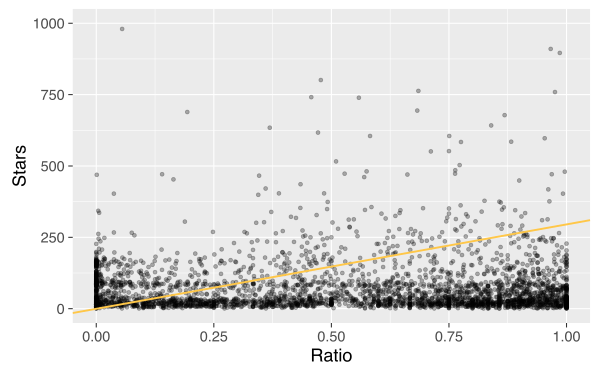
\includegraphics[page=1,scale=0.6]{../hypotheses/h3/ratio_subscriber_model_1.pdf}
	\captionof{figure}{Correlation coefficient (yellow slope) of "Ratio" on "Stars" (Model 3.1)}
	\label{fig:hyp3_m3.1}
\end{center}

\begin{landscape}
\subsubsection{H 3.1: Regression Tables}


\begin{table}[!h]
	\centering
	\scriptsize{
  	
% Table created by stargazer v.5.2 by Marek Hlavac, Harvard University. E-mail: hlavac at fas.harvard.edu
% Date and time: Sun, Mar 20, 2016 - 23:41:57
\begin{tabular}{@{\extracolsep{5pt}}lcccccccccccc}
\\[-1.8ex]\hline
\hline \\[-1.8ex]
 & \multicolumn{12}{c}{\textit{Dependent variable:}} \\
\cline{2-13}
\\[-1.8ex] & \multicolumn{4}{c}{Stars} & \multicolumn{4}{c}{Subscribers} & \multicolumn{4}{c}{Forks} \\
\\[-1.8ex] & (3.1) & (3.2) & (3.3) & (3.4) & (3.5) & (3.6) & (3.7) & (3.8) & (3.9) & (3.10) & (3.11) & (3.12)\\
\hline \\[-1.8ex]
 Ratio & 295.609$^{***}$ & 278.398$^{***}$ & 129.899 & 152.407$^{*}$ & 7.184 & 7.068 & 18.616$^{***}$ & 17.985$^{***}$ & 51.697$^{***}$ & 39.361$^{**}$ & 26.293 & 29.970 \\
  & (75.069) & (79.011) & (83.121) & (83.466) & (6.010) & (6.284) & (6.284) & (6.322) & (18.318) & (19.329) & (20.865) & (21.002) \\
  & & & & & & & & & & & & \\
 Age & 0.367$^{***}$ & 0.437$^{***}$ & 0.443$^{***}$ & 0.494$^{***}$ & 0.031$^{***}$ & 0.036$^{***}$ & 0.037$^{***}$ & 0.039$^{***}$ & 0.129$^{***}$ & 0.143$^{***}$ & 0.151$^{***}$ & 0.158$^{***}$ \\
  & (0.047) & (0.049) & (0.050) & (0.051) & (0.004) & (0.004) & (0.004) & (0.004) & (0.011) & (0.012) & (0.013) & (0.013) \\
  & & & & & & & & & & & & \\
 Constant & $-$0.236 & $-$70.590 & $-$434.208$^{***}$ & $-$764.217$^{***}$ & 48.363$^{***}$ & 47.700$^{***}$ & $-$20.544$^{*}$ & $-$39.926$^{***}$ & $-$23.486 & $-$43.139 & $-$113.655$^{***}$ & $-$192.851$^{***}$ \\
  & (60.212) & (154.968) & (139.704) & (195.611) & (4.821) & (12.325) & (10.562) & (14.817) & (14.692) & (37.910) & (35.069) & (49.222) \\
  & & & & & & & & & & & & \\
\hline \\[-1.8ex]
Observations & 3,419 & 3,419 & 3,419 & 3,419 & 3,419 & 3,419 & 3,419 & 3,419 & 3,419 & 3,419 & 3,419 & 3,419 \\
Log Likelihood & $-$29,905.750 & $-$29,877.320 & $-$29,692.650 & $-$29,668.010 & $-$21,273.000 & $-$21,221.860 & $-$20,863.760 & $-$20,845.730 & $-$25,083.110 & $-$25,063.340 & $-$24,966.870 & $-$24,950.480 \\
Akaike Inf. Crit. & 59,817.500 & 59,778.650 & 59,505.300 & 59,474.010 & 42,552.000 & 42,467.720 & 41,847.520 & 41,829.460 & 50,172.220 & 50,150.680 & 50,053.740 & 50,038.950 \\
\hline
\hline \\[-1.8ex]
\textit{Note:}  & \multicolumn{12}{r}{$^{*}$p$<$0.1; $^{**}$p$<$0.05; $^{***}$p$<$0.01} \\
\end{tabular}

	}
	\caption{Impact of "Age" and "Ratio" on "Stars", "Subscribers" and "Forks" through \textit{Fitting Generalized Linear Models} with dummy variables for \textit{Firms} and \textit{Programming Languages}. Using (a) dummy variables for each \textit{Firm} in model 3.3, 3.7 and 3.11 (b) dummy variables for each \textit{Language} in model 3.2, 3.6, 3.10 (c) dummy variables for each \textit{Firm and Language} in model 3.4, 3.8 and 3.12}
  \label{tbl:statistics_glm_project_popularity_short}
\end{table}

\begin{table}[!h]
	\centering
	\scriptsize{
  	
% Table created by stargazer v.5.2 by Marek Hlavac, Harvard University. E-mail: hlavac at fas.harvard.edu
% Date and time: Mon, Mar 21, 2016 - 00:04:00
\begin{tabular}{@{\extracolsep{5pt}}lcccccccccccc}
\\[-1.8ex]\hline
\hline \\[-1.8ex]
 & \multicolumn{12}{c}{\textit{Dependent variable:}} \\
\cline{2-13}
\\[-1.8ex] & \multicolumn{4}{c}{Number of Issues} & \multicolumn{4}{c}{Number of Contributors} & \multicolumn{4}{c}{Top Project} \\
\\[-1.8ex] & \multicolumn{4}{c}{\textit{normal}} & \multicolumn{4}{c}{\textit{normal}} & \multicolumn{4}{c}{\textit{logistic}} \\
\\[-1.8ex] & (3.13) & (3.14) & (3.15) & (3.16) & (3.17) & (3.18) & (3.19) & (3.20) & (3.21) & (3.22) & (3.23) & (3.24)\\
\hline \\[-1.8ex]
% \endhead
 Ratio & 2.147 & 2.006 & 7.861$^{*}$ & 7.612$^{*}$ & $-$2.417 & $-$2.647 & 1.391 & 1.402 & 2.025$^{***}$ & 1.727$^{***}$ & 1.906$^{***}$ & 1.753$^{***}$ \\
  & (3.717) & (3.930) & (4.235) & (4.275) & (1.911) & (2.005) & (2.051) & (2.067) & (0.155) & (0.166) & (0.191) & (0.197) \\
  & & & & & & & & & & & & \\
 Age & 0.015$^{***}$ & 0.017$^{***}$ & 0.021$^{***}$ & 0.022$^{***}$ & 0.018$^{***}$ & 0.019$^{***}$ & 0.020$^{***}$ & 0.021$^{***}$ & 0.001$^{***}$ & 0.001$^{***}$ & 0.001$^{***}$ & 0.001$^{***}$ \\
  & (0.002) & (0.002) & (0.003) & (0.003) & (0.001) & (0.001) & (0.001) & (0.001) & (0.0001) & (0.0001) & (0.0001) & (0.0001) \\
  & & & & & & & & & & & & \\
 Constant & 8.443$^{***}$ & $-$2.780 & $-$19.593$^{***}$ & $-$34.006$^{***}$ & 5.114$^{***}$ & 4.488 & $-$14.598$^{***}$ & $-$20.129$^{***}$ & $-$3.426$^{***}$ & $-$2.546$^{***}$ & $-$5.820$^{***}$ & $-$6.276$^{***}$ \\
  & (2.981) & (7.707) & (7.118) & (10.018) & (1.533) & (3.933) & (3.447) & (4.845) & (0.140) & (0.251) & (0.437) & (0.529) \\
  & & & & & & & & & & & & \\
\hline \\[-1.8ex]
Observations & 3,419 & 3,419 & 3,419 & 3,419 & 3,419 & 3,419 & 3,419 & 3,419 & 3,419 & 3,419 & 3,419 & 3,419 \\
Log Likelihood & $-$19,630.080 & $-$19,616.630 & $-$19,514.800 & $-$19,507.690 & $-$17,355.340 & $-$17,316.430 & $-$17,035.330 & $-$17,023.880 & $-$1,458.752 & $-$1,373.897 & $-$1,208.251 & $-$1,150.787 \\
Akaike Inf. Crit. & 39,266.160 & 39,257.260 & 39,149.610 & 39,153.370 & 34,716.680 & 34,656.870 & 34,190.660 & 34,185.760 & 2,923.504 & 2,771.795 & 2,536.502 & 2,439.574 \\
\hline
\hline \\[-1.8ex]
\textit{Note:}  & \multicolumn{12}{r}{$^{*}$p$<$0.1; $^{**}$p$<$0.05; $^{***}$p$<$0.01} \\
\end{tabular}

	}
	\caption{Impact of "Age" and "Ratio" on "Issues", "Contributors" and "Popularity" through \textit{Fitting Generalized Linear Models}. Using (a) dummy variables for each \textit{Firm} in model 3.15, 3.19 and 3.23 (b) dummy variables for each \textit{Language} in model 3.14, 3.18, 3.22 (c) dummy variables for each \textit{Firm and Language} in model 3.16, 3.20 and 3.24}
  \label{tbl:statistics_glm_project_popularity_short2}
\end{table}

\begin{table}
	\centering
	\footnotesize{
	  
% Table created by stargazer v.5.2 by Marek Hlavac, Harvard University. E-mail: hlavac at fas.harvard.edu
% Date and time: Mon, Mar 14, 2016 - 14:37:24
\begin{tabular}{@{\extracolsep{5pt}}lcccccc}
\\[-1.8ex]\hline
\hline \\[-1.8ex]
 & \multicolumn{6}{c}{\textit{Dependent variable:}} \\
\cline{2-7}
\\[-1.8ex] & Stars & Subscribers & Forks & Number of Issues & Number of Contributors & Top Project \\
\\[-1.8ex] & \textit{linear} & \textit{linear} & \textit{linear} & \textit{linear} & \textit{linear} & \textit{generalized linear} \\
 & \textit{mixed-effects} & \textit{mixed-effects} & \textit{mixed-effects} & \textit{mixed-effects} & \textit{mixed-effects} & \textit{mixed-effects} \\
\\[-1.8ex] & (3.25) & (3.26) & (3.27) & (3.28) & (3.29) & (3.30)\\
\hline \\[-1.8ex]
 Ratio & 149.245$^{*}$ & 18.379$^{***}$ & 31.783 & 5.896 & 1.235 & 1.910$^{***}$ \\
  & (82.032) & (6.237) & (20.266) & (4.111) & (2.032) & (0.185) \\
  & & & & & & \\
 Age & 0.420$^{***}$ & 0.036$^{***}$ & 0.142$^{***}$ & 0.020$^{***}$ & 0.020$^{***}$ & 0.001$^{***}$ \\
  & (0.049) & (0.004) & (0.012) & (0.002) & (0.001) & (0.0001) \\
  & & & & & & \\
 Constant & 160.468 & 44.443$^{***}$ & $-$9.606 & 2.911 & 2.225 & $-$3.497$^{***}$ \\
  & (104.513) & (9.753) & (21.187) & (4.280) & (2.974) & (0.235) \\
  & & & & & & \\
\hline \\[-1.8ex]
Observations & 3,419 & 3,419 & 3,419 & 3,419 & 3,419 & 3,419 \\
Log Likelihood & $-$29,774.830 & $-$20,966.900 & $-$25,031.110 & $-$19,582.970 & $-$17,137.260 & $-$1,298.686 \\
Akaike Inf. Crit. & 59,559.660 & 41,943.800 & 50,072.220 & 39,175.940 & 34,284.520 & 2,605.372 \\
Bayesian Inf. Crit. & 59,590.340 & 41,974.490 & 50,102.910 & 39,206.620 & 34,315.210 & 2,629.921 \\
\hline
\hline \\[-1.8ex]
\textit{Note:}  & \multicolumn{6}{r}{$^{*}$p$<$0.1; $^{**}$p$<$0.05; $^{***}$p$<$0.01} \\
\end{tabular}

	}
	\caption{Impact of "Age" and "Ratio" on projects' social metrics ("Stars", "Subscribers", "Forks" and "Issues") and popularity (is "Top Project" yes / no) through \textit{Mixed Model} between \textit{Firms}. "Number of Contributors" is just a control attribute and not a describing model.}
	\label{tbl:h3.1_mixed_models_popularity}
\end{table}

See regression table \ref{tbl:lmer_ratio_as_dependent_1} and \ref{tbl:lmer_ratio_as_dependent_2} (page \pageref{tbl:lmer_ratio_as_dependent_1} - \pageref{tbl:lmer_ratio_as_dependent_2}) for results having "Ratio" as dependent variable and table \ref{tbl:h3.1_mixed_models_size} (page \pageref{tbl:h3.1_mixed_models_size}) for \textit{Mixed Model} between Firms and Programming Languages.

\end{landscape}

\clearpage
\normalsize

\subsection{H 3: Results and Interpretation}

\textbf{The "Ratio" (i.e. the share of code commits by firm employed developers) has a significant positive impact on the popularity of a project.}

If we use "Stars" as a proxy for popularity, we can approve that the "Ratio" has a high positive influence on the likelihood that a project is (very) popular (correlation coefficient is 295, see model 3.1 in table \ref{tbl:statistics_glm_project_popularity_short}). This extends to "Subscribers" as well but with a lower impact (see model 3.7 and 3.8 in table \ref{tbl:statistics_glm_project_popularity_short}). "Forks" are also positively influenced by "Ratio" but also with a much lower correlation coefficient (see model 3.10 in table \ref{tbl:statistics_glm_project_popularity_short}). Interestingly enough, "Ratio" has no (significant) impact on the number of issues - but issue participation share has an impact on success and popularity (as shown in chapter \ref{sec:h1.2_h1.3_results_and_interpretation}).

Unfortunately, dummy variables (for \textit{Firms} and \textit{Programming Languages} respectively) have diverse effects on the regression results. This might be caused by different popularity attributes which are effected by different users' behavior. For example: \textit{JavaScript} developers could be more "Stargazer" friendly, \textit{C++} developer user more "Subscriber" friendly (and so on). Firms also may have different effects on specific popularity attributes: Some are more popular and some are less popular in the OS community (see the example of \textit{Microsoft} and \textit{GitHub} in chapter \ref{sec:atom_vs_vsc}).

Another broad hint is given by the \textit{logistic regression models}: \textbf{The probability that a project is a "Top Project" depends significant on the size of "Ratio"} (see model 3.21 - 3.24 in table \ref{tbl:statistics_glm_project_popularity_short2}). By using logistics regression we can interpret $\beta_{j}$ through $e^{\beta{j}}$ as effect coefficient \cite[p. 71]{agresti2007introduction}. Thus, the effect coefficient is between $e^{1.727} \approx 5.62$ and $e^{1.91} \approx 6.75$ \footnote{the problem of multicollinearity might reduce the validity of the mentioned effect coefficients, but seems to be rejected by results in observations over time (see chapter \ref{sec:h2_analysis})}.
 \textbf{This means that projects with highest "Ratios" are more likely "Top Projects" by the factor of 6.}
